

Такой класс моделей

Вариационные кодировщики класс вероятностных моделей, использующие промежуточное скрытое представление.

Предшественником подхода вариационного кодировщика был автокодировщик, состоящий из двух частей: \begin{enumerate}
    \item модель компрессии изначального изображения $g_\phi$;
    \item модель декомпрессии изначального изображения $f_\theta$.
\end{enumerate}

\begin{figure}[h]
    \centering
    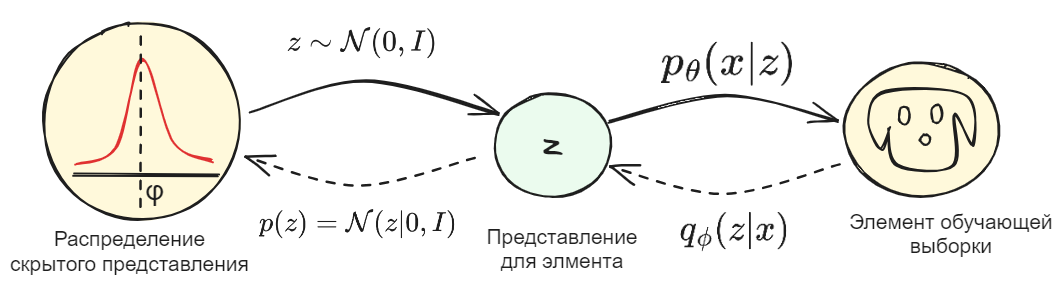
\includegraphics[width=0.5\textwidth]{assets/ml/generation/vae.excalidraw.png}
    \caption{Вариационный кодировщик задает ошибку кодирования в виде параметрического нормального распределения}
    \label{discr_vs_gen}
\end{figure}
Функция оптимизации такой модели записывается как среднеквадратичная разность между входом и выходом модели:
\begin{equation}
    L_\text{AE}(\theta, \phi) = \frac{1}{n}\sum_{i=1}^n (\mathbf{x}^{(i)} - f_\theta(g_\phi(\mathbf{x}^{(i)})))^2
\end{equation}
Аппарат автокодировщика может быть усовершенствован путем учета распределения ошибки кодирования. В предметной области
преимущественно используются параметрические распределения $p_\theta$, поскольку они могут быть численно адаптированы под 
произвольную постановку при наличии достаточного числа данных. Поиск параметров выполняется путем вариации функционала:
\begin{equation}
    -L_\text{VAE} = \log p_\theta(\mathbf{x}) - D_\text{KL}( q_\phi(\mathbf{z}\vert\mathbf{x}) \| p_\theta(\mathbf{z}\vert\mathbf{x}) ) \leq \log p_\theta(\mathbf{x})
\end{equation}
В работе \cite{kingma2013auto} предложен численно эффективный учет ошибки заданный нормальным распределения.
Обучение происходит путем автоматического дифференцирования по параметрам распределения: 
\begin{equation}
    \begin{aligned}
        \mathbf{z} &\sim q_\phi(\mathbf{z}\vert\mathbf{x}^{(i)}) = \mathcal{N}(\mathbf{z}; \boldsymbol{\mu}^{(i)}, \boldsymbol{\sigma}^{2(i)}\boldsymbol{I}) & \\
        \mathbf{z} &= \boldsymbol{\mu} + \boldsymbol{\sigma} \boldsymbol{\epsilon},
    \end{aligned}
\end{equation}
, где $\boldsymbol{\epsilon} \sim \mathcal{N}(0, \boldsymbol{I})$. Функция оптимизации с учетом репараметризации запишется как:
\begin{equation}
    \max_{\phi, \theta} \mathbb{E}_{\mathbf{x}\sim\mathcal{D}}[\mathbb{E}_{\mathbf{z} \sim q_\phi(\mathbf{z}\vert\mathbf{x})} \log p_\theta(\mathbf{x}\vert\mathbf{z})]
\end{equation}
c регуляризационным условием на дивергенцию $D_\text{KL}(q_\phi(\mathbf{z}\vert\mathbf{x})\|p_\theta(\mathbf{z})) < \delta$ для обучения декодировщика. 
Тогда оптимизационный Лангражиан $\mathcal{L}$ с множителем $\beta$ для условия запишется как:
\begin{equation}
    \begin{aligned}
        \mathcal{L}(\theta, \phi, \beta) &= \mathbb{E}_{\mathbf{z} \sim q_\phi(\mathbf{z}\vert\mathbf{x})} \log p_\theta(\mathbf{x}\vert\mathbf{z}) - \beta(D_\text{KL}(q_\phi(\mathbf{z}\vert\mathbf{x})\|p_\theta(\mathbf{z})) - \delta) & \\
        & = \mathbb{E}_{\mathbf{z} \sim q_\phi(\mathbf{z}\vert\mathbf{x})} \log p_\theta(\mathbf{x}\vert\mathbf{z}) - \beta D_\text{KL}(q_\phi(\mathbf{z}\vert\mathbf{x})\|p_\theta(\mathbf{z})) + \beta \delta & \\
        & \geq \mathbb{E}_{\mathbf{z} \sim q_\phi(\mathbf{z}\vert\mathbf{x})} \log p_\theta(\mathbf{x}\vert\mathbf{z}) - \beta D_\text{KL}(q_\phi(\mathbf{z}\vert\mathbf{x})\|p_\theta(\mathbf{z}))
    \end{aligned}
\end{equation}
Итоговая оптимизационная функция с гиперпараметром $\beta$ записывается как:
$$
L_\text{BETA}(\phi, \beta) = - \mathbb{E}_{\mathbf{z} \sim q_\phi(\mathbf{z}\vert\mathbf{x})} \log p_\theta(\mathbf{x}\vert\mathbf{z}) + \beta D_\text{KL}(q_\phi(\mathbf{z}\vert\mathbf{x})\|p_\theta(\mathbf{z}))
$$

Вариационные кодировщики позволяют лишь выполнить оценку снизу на плотность вероятностной массы.
Получения вероятности в явной форме можно выполнить, используя модели потоков.

\textit{Определение } \textbf{Модели нормализационных потоков} называют генеративные модели основанные 
на последовательных обратимых дифференцируемых преобразованиях. \footnote{"Нормальность" потока связана с явным введением параметра сжатия фазового объема 
в выражение}
\begin{equation}
    \log p_{K}(z_K) = \log p_0(z_0) - \sum_{i=1}^K \log \left|\det \frac{d f_i(z_{i-1})}{d z_{i-1}} \right| 
\end{equation}

Обратимые дифференцируемые преобразования позволяют использовать теорему о замене переменных для связи плотности вероятности в ходе преобразований:
\begin{equation}
    \begin{aligned}
        \mathbf{z} &\sim \pi(\mathbf{z}), \mathbf{x} = f(\mathbf{z}), \mathbf{z} = f^{-1}(\mathbf{x}) \\
        p(\mathbf{x}) 
        &= \pi(\mathbf{z}) \left\vert \det \dfrac{d \mathbf{z}}{d \mathbf{x}} \right\vert  
        = \pi(f^{-1}(\mathbf{x})) \left\vert \det \dfrac{d f^{-1}}{d \mathbf{x}} \right\vert,
    \end{aligned}
\end{equation}
где $\det \frac{\partial f}{\partial\mathbf{z}}$ якобиан функции $f$.

\begin{figure}[h]
    \centering
    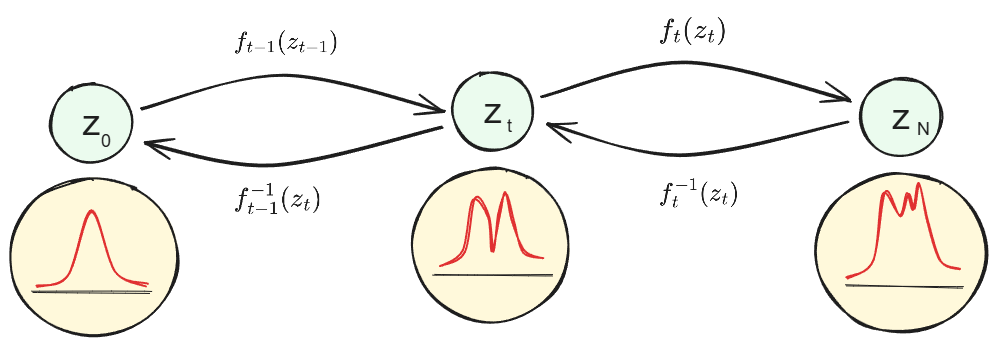
\includegraphics[width=0.5\textwidth]{assets/ml/generation/flow.excalidraw.png}
    \caption{Модели потока используют последовательные обратимые преобразования для приведения исследуемого распределения к известному}
    \label{flow}
\end{figure}

Ключевым для численной разрешимости постановки является простота вычисления логарифма детерминанта и невырожденность $\det \frac{d f_i(z_{i-1})}{d z_{i-1}}$. 
Для исследований класса функции с заданными требованиями как правило используются перестановки слагаемых и матричные преобразования.

RealNVP

В качестве преобразования предлагается афинное преобразование последних $D-d$ компонент вектора генерации:  

\begin{equation}
    \begin{aligned}
        \mathbf{y}_{1:d} &= \mathbf{x}_{1:d} \\ 
        \mathbf{y}_{d+1:D} &= \mathbf{x}_{d+1:D} \odot \exp({s(\mathbf{x}_{1:d})}) + t(\mathbf{x}_{1:d})
    \end{aligned}
\end{equation}

Детерминант полученного выражения запишется как:

\begin{equation}
    \mathbf{J} = 
    \begin{bmatrix}
    \mathbb{I}_d & \mathbf{0}_{d\times(D-d)} \\[5pt]
    \frac{\partial \mathbf{y}_{d+1:D}}{\partial \mathbf{x}_{1:d}} & \text{diag}(\exp(s(\mathbf{x}_{1:d})))
    \end{bmatrix}
\end{equation}

Авторы подхода NICE предложили использовать одномерные сверточные слои по сути являющимися функциями сдвига и масштабирования:

\begin{equation}
    \begin{cases}
    \mathbf{y}_{1:d} &= \mathbf{x}_{1:d} \\ 
    \mathbf{y}_{d+1:D} &= \mathbf{x}_{d+1:D} + m(\mathbf{x}_{1:d})
    \end{cases}
    \Leftrightarrow 
    \begin{cases}
    \mathbf{x}_{1:d} &= \mathbf{y}_{1:d} \\ 
    \mathbf{x}_{d+1:D} &= \mathbf{y}_{d+1:D} - m(\mathbf{y}_{1:d})
    \end{cases}
\end{equation}

Логарифм детерминанта преобразования в этом случае запишется как:

\begin{equation}
    \log \left\vert\det \frac{\partial\texttt{conv2d}(\mathbf{h}; \mathbf{W})}{\partial\mathbf{h}}\right\vert
    = \log (\vert\det\mathbf{W}\vert^{h \cdot w}\vert) = h \cdot w \cdot \log \vert\det\mathbf{W}\vert
\end{equation}



